\documentclass{standalone}
\usepackage{tikz}
\usetikzlibrary{patterns, positioning}


\begin{document}
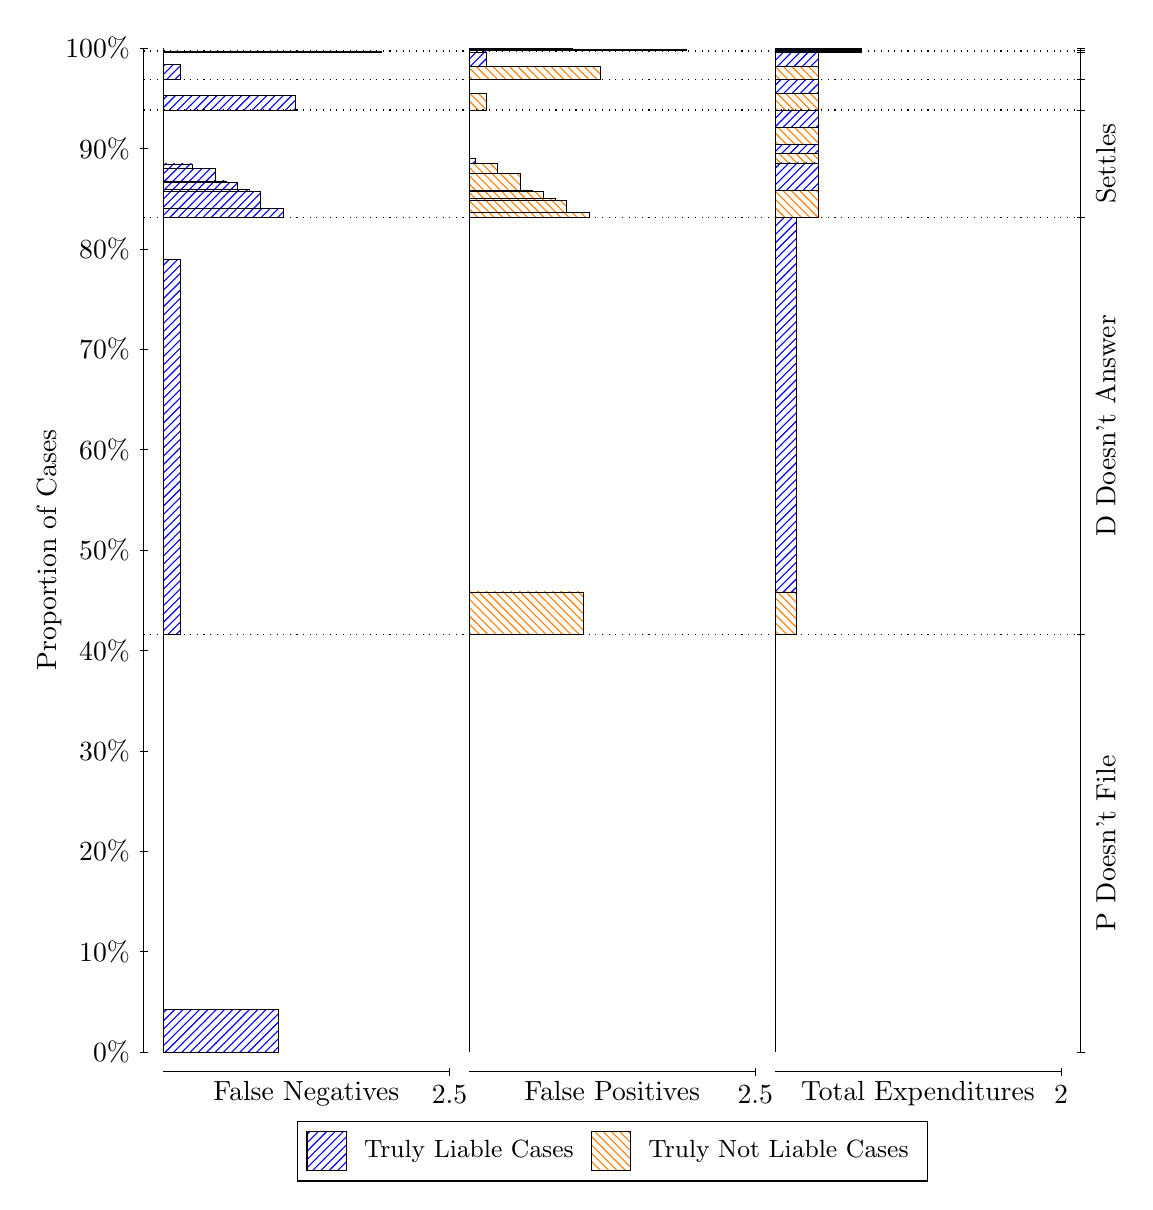
\begin{tikzpicture}
\draw[black, very thin] (1.5,1.75) -- (1.5,14.5);
\node[rotate=90, text=black, anchor=center] at (0.3, 8.125) {Proportion of Cases};
\draw[black, very thin] (1.45,1.75) -- (1.55,1.75);
\node[text=black, anchor=east] at (1.45, 1.75) {0\%};
\draw[black, very thin] (1.45,3.025) -- (1.55,3.025);
\node[text=black, anchor=east] at (1.45, 3.025) {10\%};
\draw[black, very thin] (1.45,4.3) -- (1.55,4.3);
\node[text=black, anchor=east] at (1.45, 4.3) {20\%};
\draw[black, very thin] (1.45,5.575) -- (1.55,5.575);
\node[text=black, anchor=east] at (1.45, 5.575) {30\%};
\draw[black, very thin] (1.45,6.85) -- (1.55,6.85);
\node[text=black, anchor=east] at (1.45, 6.85) {40\%};
\draw[black, very thin] (1.45,8.125) -- (1.55,8.125);
\node[text=black, anchor=east] at (1.45, 8.125) {50\%};
\draw[black, very thin] (1.45,9.4) -- (1.55,9.4);
\node[text=black, anchor=east] at (1.45, 9.4) {60\%};
\draw[black, very thin] (1.45,10.675) -- (1.55,10.675);
\node[text=black, anchor=east] at (1.45, 10.675) {70\%};
\draw[black, very thin] (1.45,11.95) -- (1.55,11.95);
\node[text=black, anchor=east] at (1.45, 11.95) {80\%};
\draw[black, very thin] (1.45,13.225) -- (1.55,13.225);
\node[text=black, anchor=east] at (1.45, 13.225) {90\%};
\draw[black, very thin] (1.45,14.5) -- (1.55,14.5);
\node[text=black, anchor=east] at (1.45, 14.5) {100\%};

\draw[black, very thin] (13.4,1.75) -- (13.4,14.5);
\draw[black, very thin] (13.35,1.75) -- (13.45,1.75);
\node[anchor=west] at (13.35, 1.75) {};
\draw[black, very thin] (13.35,7.0516) -- (13.45,7.0516);
\node[anchor=west] at (13.35, 7.0516) {};
\draw[black, very thin] (13.35,12.352) -- (13.45,12.352);
\node[anchor=west] at (13.35, 12.352) {};
\draw[black, very thin] (13.35,13.713) -- (13.45,13.713);
\node[anchor=west] at (13.35, 13.713) {};
\draw[black, very thin] (13.35,14.103) -- (13.45,14.103);
\node[anchor=west] at (13.35, 14.103) {};
\draw[black, very thin] (13.35,14.451) -- (13.45,14.451);
\node[anchor=west] at (13.35, 14.451) {};
\draw[black, very thin] (13.35,14.473) -- (13.45,14.473);
\node[anchor=west] at (13.35, 14.473) {};
\draw[black, very thin] (13.35,14.5) -- (13.45,14.5);
\node[anchor=west] at (13.35, 14.5) {};

\draw[black, very thin, pattern color=blue, pattern=north east lines] (1.75,1.75) rectangle (3.2033,2.2912);
\draw[black, very thin, pattern color=orange, pattern=north west lines] (1.75,2.2912) rectangle (1.75,7.0516);
\draw[black, very thin, pattern color=blue, pattern=north east lines] (1.75,7.0516) rectangle (1.968,11.811);
\draw[black, very thin, pattern color=orange, pattern=north west lines] (1.75,11.811) rectangle (1.75,12.352);
\draw[black, very thin, pattern color=blue, pattern=north east lines] (1.75,12.352) rectangle (3.276,12.467);
\draw[black, very thin, pattern color=blue, pattern=north east lines] (1.75,12.467) rectangle (2.9853,12.684);
\draw[black, very thin, pattern color=blue, pattern=north east lines] (1.75,12.684) rectangle (2.84,12.703);
\draw[black, very thin, pattern color=blue, pattern=north east lines] (1.75,12.703) rectangle (2.6947,12.792);
\draw[black, very thin, pattern color=blue, pattern=north east lines] (1.75,12.792) rectangle (2.5493,12.812);
\draw[black, very thin, pattern color=blue, pattern=north east lines] (1.75,12.812) rectangle (2.404,12.968);
\draw[black, very thin, pattern color=blue, pattern=north east lines] (1.75,12.968) rectangle (2.1133,13.03);
\draw[black, very thin, pattern color=orange, pattern=north west lines] (1.75,13.03) rectangle (1.75,13.713);
\draw[black, very thin, pattern color=blue, pattern=north east lines] (1.75,13.713) rectangle (3.4213,13.897);
\draw[black, very thin, pattern color=orange, pattern=north west lines] (1.75,13.897) rectangle (1.75,14.103);
\draw[black, very thin, pattern color=blue, pattern=north east lines] (1.75,14.103) rectangle (1.968,14.289);
\draw[black, very thin, pattern color=orange, pattern=north west lines] (1.75,14.289) rectangle (1.75,14.451);
\draw[black, very thin, pattern color=blue, pattern=north east lines] (1.75,14.451) rectangle (4.5113,14.46);
\draw[black, very thin, pattern color=orange, pattern=north west lines] (1.75,14.46) rectangle (1.75,14.473);
\draw[black, very thin, pattern color=orange, pattern=north west lines] (1.75,14.473) rectangle (1.75,14.483);
\draw[black, very thin, pattern color=blue, pattern=north east lines] (1.75,14.483) rectangle (1.75,14.5);
\draw[black, very thin, pattern color=orange, pattern=north west lines] (5.6333,1.75) rectangle (5.6333,6.5104);
\draw[black, very thin, pattern color=blue, pattern=north east lines] (5.6333,6.5104) rectangle (5.6333,7.0516);
\draw[black, very thin, pattern color=orange, pattern=north west lines] (5.6333,7.0516) rectangle (7.0867,7.5922);
\draw[black, very thin, pattern color=blue, pattern=north east lines] (5.6333,7.5922) rectangle (5.6333,12.352);
\draw[black, very thin, pattern color=orange, pattern=north west lines] (5.6333,12.352) rectangle (7.1593,12.41);
\draw[black, very thin, pattern color=orange, pattern=north west lines] (5.6333,12.41) rectangle (6.8687,12.566);
\draw[black, very thin, pattern color=orange, pattern=north west lines] (5.6333,12.566) rectangle (6.7233,12.586);
\draw[black, very thin, pattern color=orange, pattern=north west lines] (5.6333,12.586) rectangle (6.578,12.675);
\draw[black, very thin, pattern color=orange, pattern=north west lines] (5.6333,12.675) rectangle (6.4327,12.694);
\draw[black, very thin, pattern color=orange, pattern=north west lines] (5.6333,12.694) rectangle (6.2873,12.911);
\draw[black, very thin, pattern color=orange, pattern=north west lines] (5.6333,12.911) rectangle (5.9967,13.034);
\draw[black, very thin, pattern color=blue, pattern=north east lines] (5.6333,13.034) rectangle (5.706,13.096);
\draw[black, very thin, pattern color=blue, pattern=north east lines] (5.6333,13.096) rectangle (5.6333,13.713);
\draw[black, very thin, pattern color=orange, pattern=north west lines] (5.6333,13.713) rectangle (5.8513,13.919);
\draw[black, very thin, pattern color=blue, pattern=north east lines] (5.6333,13.919) rectangle (5.6333,14.103);
\draw[black, very thin, pattern color=orange, pattern=north west lines] (5.6333,14.103) rectangle (7.3047,14.265);
\draw[black, very thin, pattern color=blue, pattern=north east lines] (5.6333,14.265) rectangle (5.8513,14.451);
\draw[black, very thin, pattern color=orange, pattern=north west lines] (5.6333,14.451) rectangle (5.6333,14.465);
\draw[black, very thin, pattern color=blue, pattern=north east lines] (5.6333,14.465) rectangle (5.6333,14.473);
\draw[black, very thin, pattern color=orange, pattern=north west lines] (5.6333,14.473) rectangle (8.3947,14.483);
\draw[black, very thin, pattern color=blue, pattern=north east lines] (5.6333,14.483) rectangle (6.9413,14.5);
\draw[black, very thin, pattern color=orange, pattern=north west lines] (9.5167,1.75) rectangle (9.5167,6.5104);
\draw[black, very thin, pattern color=blue, pattern=north east lines] (9.5167,6.5104) rectangle (9.5167,7.0516);
\draw[black, very thin, pattern color=orange, pattern=north west lines] (9.5167,7.0516) rectangle (9.7892,7.5922);
\draw[black, very thin, pattern color=blue, pattern=north east lines] (9.5167,7.5922) rectangle (9.7892,12.352);
\draw[black, very thin, pattern color=orange, pattern=north west lines] (9.5167,12.352) rectangle (10.062,12.694);
\draw[black, very thin, pattern color=blue, pattern=north east lines] (9.5167,12.694) rectangle (10.062,13.041);
\draw[black, very thin, pattern color=orange, pattern=north west lines] (9.5167,13.041) rectangle (10.062,13.165);
\draw[black, very thin, pattern color=blue, pattern=north east lines] (9.5167,13.165) rectangle (10.062,13.28);
\draw[black, very thin, pattern color=orange, pattern=north west lines] (9.5167,13.28) rectangle (10.062,13.496);
\draw[black, very thin, pattern color=blue, pattern=north east lines] (9.5167,13.496) rectangle (10.062,13.713);
\draw[black, very thin, pattern color=orange, pattern=north west lines] (9.5167,13.713) rectangle (10.062,13.919);
\draw[black, very thin, pattern color=blue, pattern=north east lines] (9.5167,13.919) rectangle (10.062,14.103);
\draw[black, very thin, pattern color=orange, pattern=north west lines] (9.5167,14.103) rectangle (10.062,14.265);
\draw[black, very thin, pattern color=blue, pattern=north east lines] (9.5167,14.265) rectangle (10.062,14.451);
\draw[black, very thin, pattern color=orange, pattern=north west lines] (9.5167,14.451) rectangle (10.607,14.465);
\draw[black, very thin, pattern color=blue, pattern=north east lines] (9.5167,14.465) rectangle (10.607,14.473);
\draw[black, very thin, pattern color=orange, pattern=north west lines] (9.5167,14.473) rectangle (10.607,14.483);
\draw[black, very thin, pattern color=blue, pattern=north east lines] (9.5167,14.483) rectangle (10.607,14.5);
\draw[black, dotted] (1.5,7.0516) -- (13.4,7.0516);
\draw[black, dotted] (1.5,12.352) -- (13.4,12.352);
\draw[black, dotted] (1.5,13.713) -- (13.4,13.713);
\draw[black, dotted] (1.5,14.103) -- (13.4,14.103);
\draw[black, dotted] (1.5,14.451) -- (13.4,14.451);
\draw[black, dotted] (1.5,14.473) -- (13.4,14.473);
\draw[black, very thin] (1.75,1.5) -- (5.3833,1.5);
\node[text=black, anchor=north] at (3.5667, 1.5) {False Negatives};
\draw[black, very thin] (5.3833,1.45) -- (5.3833,1.55);
\node[text=black, anchor=north] at (5.3833, 1.45) {2.5};

\draw[black, very thin] (5.6333,1.5) -- (9.2667,1.5);
\node[text=black, anchor=north] at (7.45, 1.5) {False Positives};
\draw[black, very thin] (9.2667,1.45) -- (9.2667,1.55);
\node[text=black, anchor=north] at (9.2667, 1.45) {2.5};

\draw[black, very thin] (9.5167,1.5) -- (13.15,1.5);
\node[text=black, anchor=north] at (11.333, 1.5) {Total Expenditures};
\draw[black, very thin] (13.15,1.45) -- (13.15,1.55);
\node[text=black, anchor=north] at (13.15, 1.45) {2};

\node[text=black, centered, rotate=90] at (13.72, 4.4008) {P Doesn't File};
\node[text=black, centered, rotate=90] at (13.72, 9.7018) {D Doesn't Answer};
\node[text=black, centered, rotate=90] at (13.72, 13.032) {Settles};





\draw (7.449999999999999,1.5) node[draw=none] (baseCoordinate) {};
\begin{scope}[align=center]
        \matrix[scale=0.5, draw=black, below=0.5cm of baseCoordinate, nodes={draw}, column sep=0.1cm]{
            \node[rectangle, draw, minimum width=0.5cm, minimum height=0.5cm, pattern color=blue, pattern=north east lines] {}; &
            \node[draw=none, font=\small, text=black] (B) {Truly Liable Cases}; &
            \node[rectangle, draw, minimum width=0.5cm, minimum height=0.5cm, pattern color=orange, pattern=north west lines] {}; &
            \node[draw=none, font=\small, text=black] (B) {Truly Not Liable Cases}; \\
            };
\end{scope}

\end{tikzpicture}
\end{document}